% remember to set these at the start of each chapter
\chapter{Experiments and Discussion} 
\label{experiments}
In this section, we show and discuss the performance of each CNN model, including Small CNN, VGG, VGG-IN, and ResNet. Training is performed on PAT and US dataset and two other datasets for verification. Section \ref{result_dataset} and \ref{result_aug} describe the dataset and data pre-processing. Section \ref{result_training} describes the training process, and Section \ref{result_curves} and \ref{result_acc} include the experiment results. We then have a discussion about the results in Section \ref{result_discussion}. Finally, the experimental results on other datasets are shown in Section \ref{result_other}.
%%%%%%%%%%%%%%%%%%
\section{Dataset}
\label{result_dataset}
The dataset is obtained from the study of \cite{Kosik2019}. It contains 90 breast cancer tumour samples, each of which has an Ultrasound (US) image stack and a Photoacoustic (PAT) image stack. In the dataset, each sample belongs to one of 14 types (class A - N) of cancer, where the actual cancer name is masked to obtain a blind study. The distribution of cancer classes is shown in Fig.\,\ref{class_graph}.  
\begin{figure}[h]
	\centering
	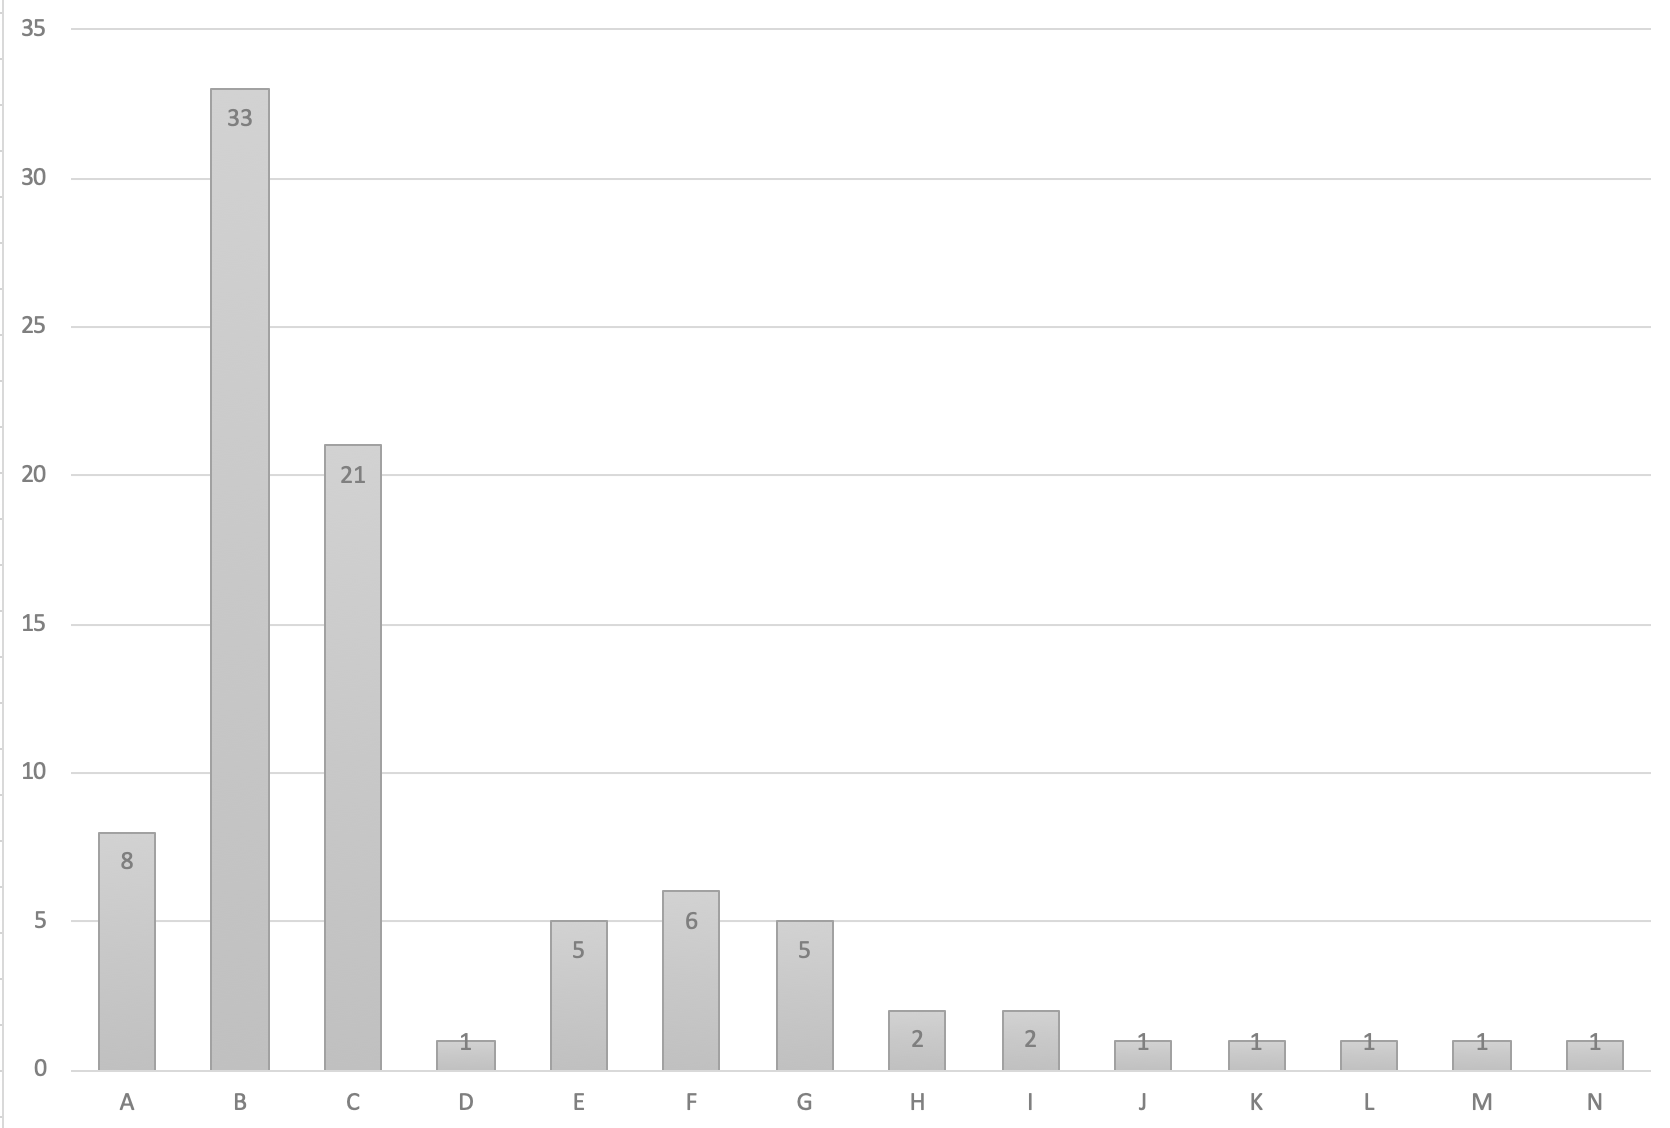
\includegraphics[width=0.7\textwidth]{Figs/class_graph.png}
    \caption{Cancer types and number of samples per type}
    \label{class_graph}
\end{figure}

B has 33 samples and C has 21 samples. In this project, only class B and C are used, because the other classes have too few samples to train a neural network.

A specimen of breast cancer tumour is scanned in the $z$ direction (vertical) relative to the holding platform. Scans produce a stack of 2D images of the cross-section. An example of an image stack is shown in Fig.\,\ref{stack}. 

\begin{figure}[h]
	\centering
	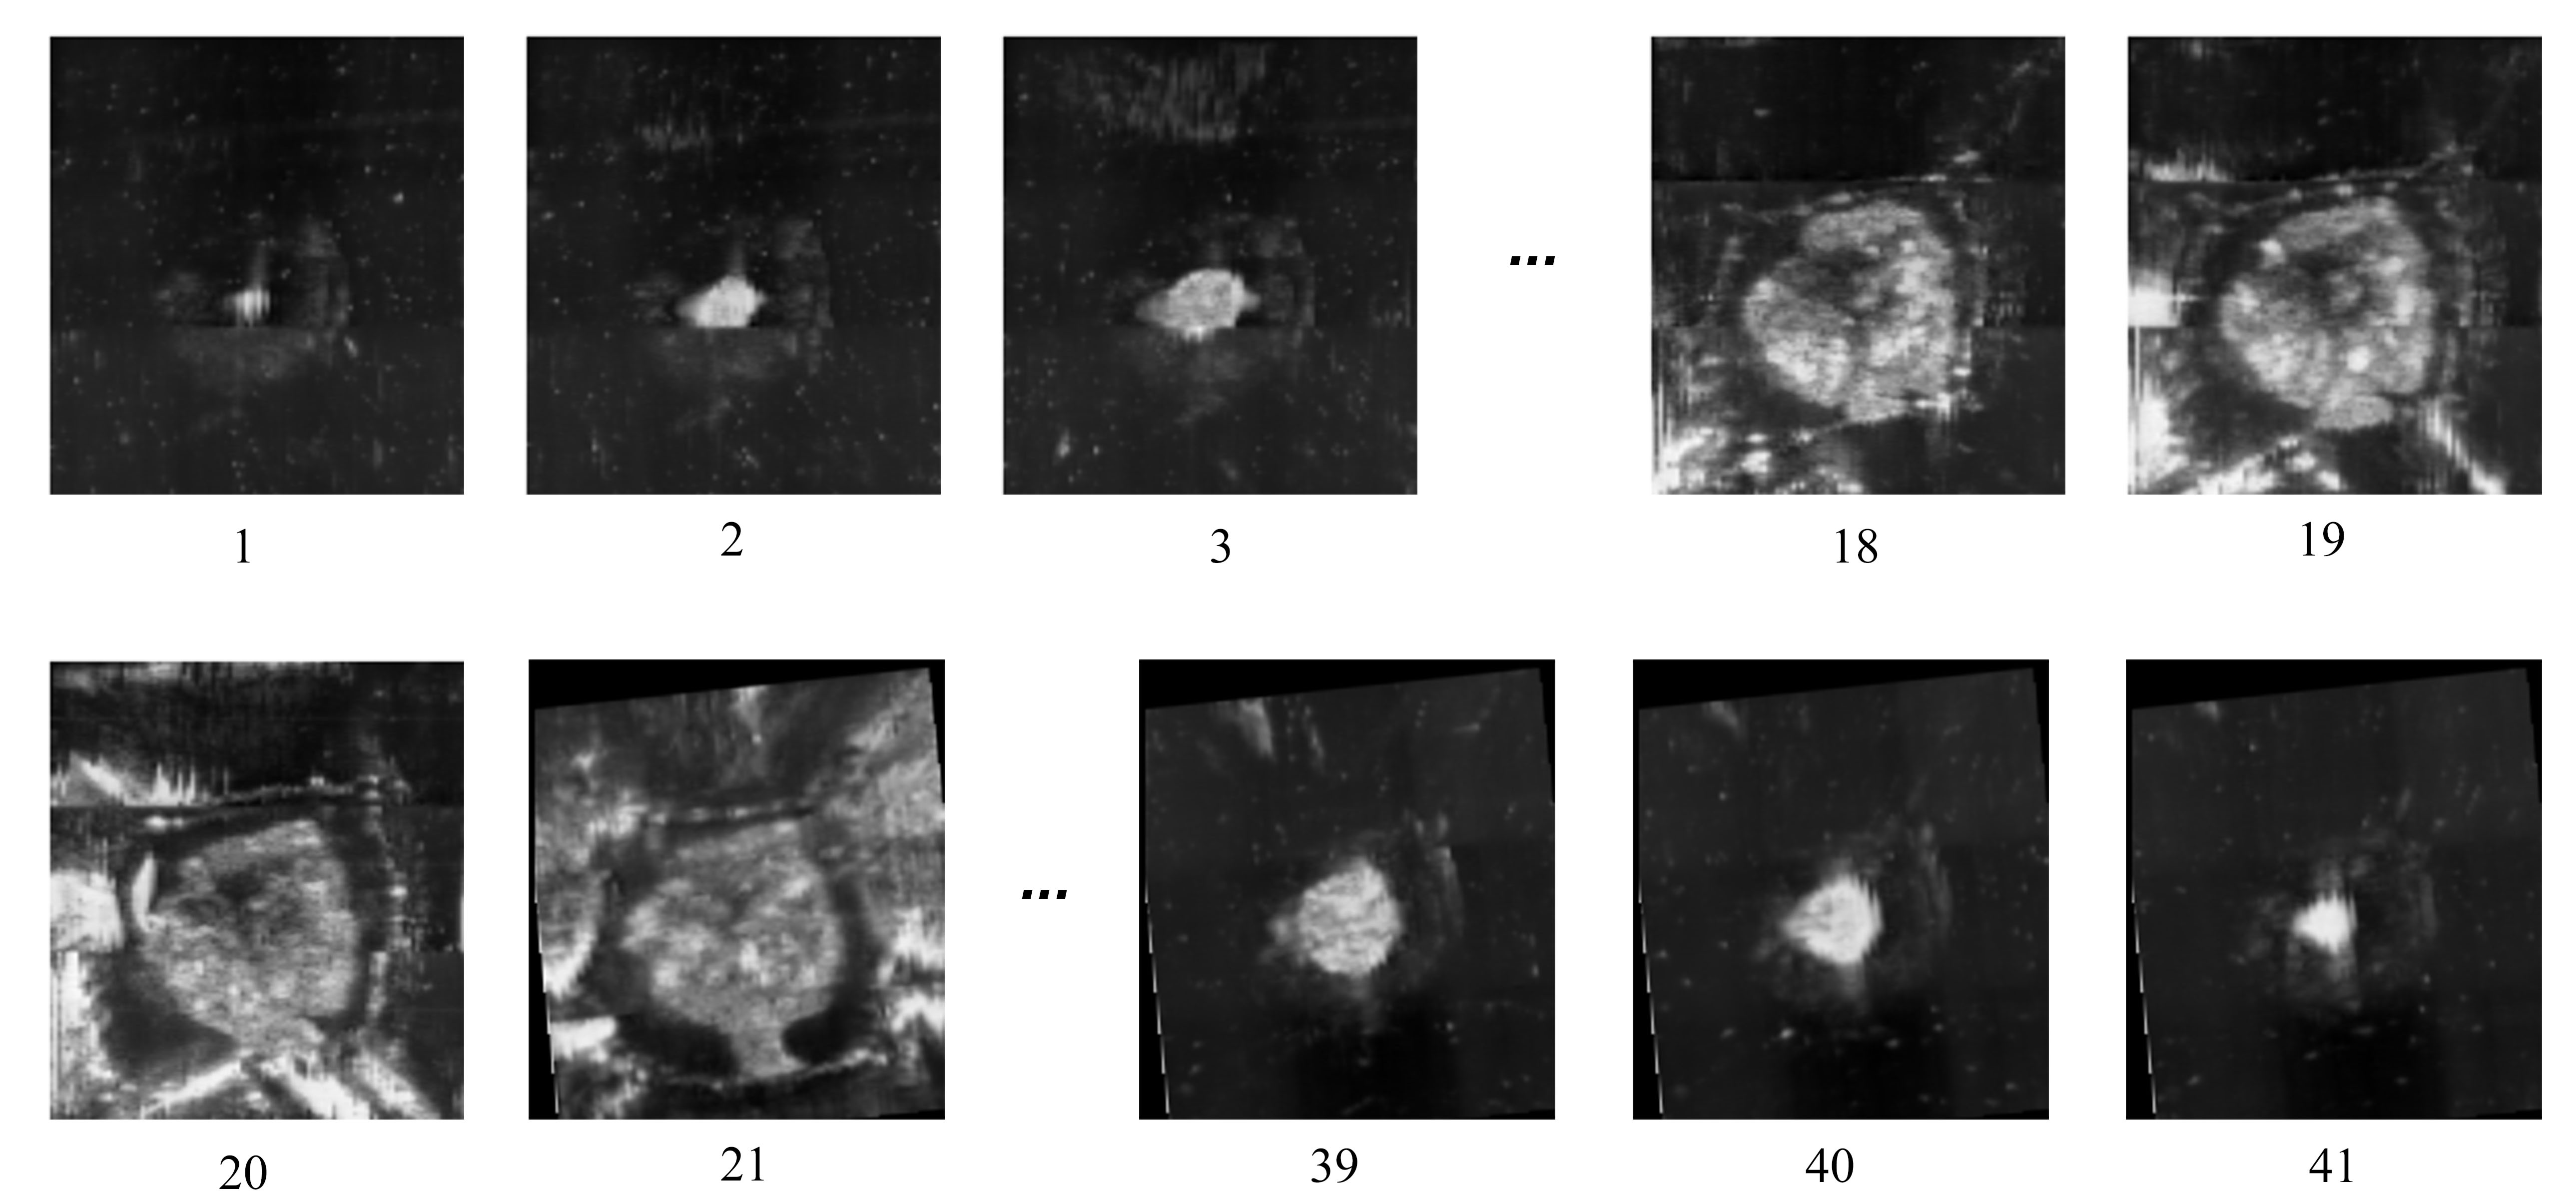
\includegraphics[width=\textwidth]{Figs/pat_stack_50.jpg}
    \caption{US stack example}
    \label{stack}
\end{figure}

We can see that the top and bottom scans, for example 1, 2, 3, 39, 40, 41 in Fig.\,\ref{stack}, are very small and lack of detail of the internal texture. This is because the cross-sections close to the top and bottom of a tumour specimen are very small. The cross-sections close to the centre of a specimen, such as 18, 19, 21, 21 are larger in size and have more texture. For each image stack, US and PAT, the centre 6 images are extracted (we could extract more or even use all of the images, but we may not want to use images with poor quality) to use for training and validation. There are in total 389 PAT images and 344 US images extracted from the stacks. Examples of extracted PAT and US images are shown in Fig.\,\ref{pat_us_example}.

\begin{figure}
\centering
\begin{subfigure}[b]{.24\linewidth}
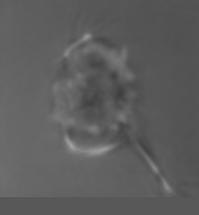
\includegraphics[width=\linewidth]{Figs/PAT014_18.jpg}
\caption{AF014 PAT}
\end{subfigure}
\begin{subfigure}[b]{.24\linewidth}
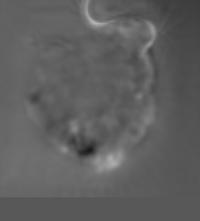
\includegraphics[width=\linewidth]{Figs/PAT023_23.jpg}
\caption{AF023 PAT}
\end{subfigure}
\begin{subfigure}[b]{.24\linewidth}
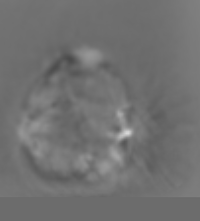
\includegraphics[width=\linewidth]{Figs/PAT36.png}
\caption{AF036 PAT}
\end{subfigure}
\begin{subfigure}[b]{.24\linewidth}
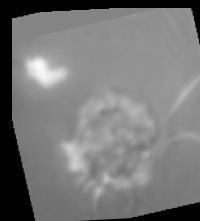
\includegraphics[width=\linewidth]{Figs/PAT055_11.jpg}
\caption{AF055 PAT}
\end{subfigure}

\begin{subfigure}[b]{.24\linewidth}
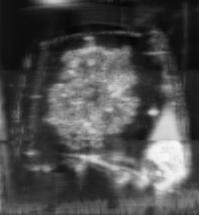
\includegraphics[width=\linewidth]{Figs/US14_18.jpg}
\caption{AF014 US}
\end{subfigure}
\begin{subfigure}[b]{.24\linewidth}
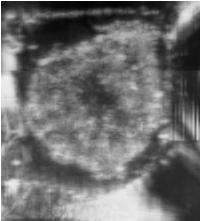
\includegraphics[width=\linewidth]{Figs/US23_23.jpg}
\caption{AF023 US}
\end{subfigure}
\begin{subfigure}[b]{.24\linewidth}
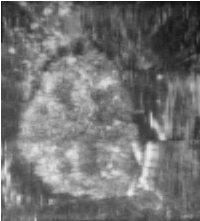
\includegraphics[width=\linewidth]{Figs/US36.png}
\caption{AF036 US}
\end{subfigure}
\begin{subfigure}[b]{.24\linewidth}
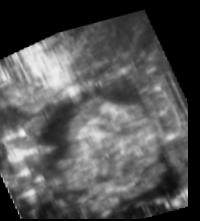
\includegraphics[width=\linewidth]{Figs/US55_13.jpg}
\caption{AF055 US}
\end{subfigure}
\caption{Extracted PAT and US images}
\label{pat_us_example}
\end{figure}

\section{Data Partition and Augmentation}
\label{result_aug}

The images are divided into a training set and a testing set by an 80/20 ratio. No image from the same stack is separated into the training and the testing set. Because the number of samples in class B and C is not balanced, K-fold data partitioning is done using a Stratified k-fold. Stratified k-fold is where the training set and the testing set contains approximately the same percentage of samples of each target class as the original dataset. Each of the five folds is used as a test set only once. Accuracy and $F_1$ score (defined as (\ref{f1_score})) are averaged across five folds.

Machine learning generally requires large amounts of data. Since our dataset is small, data augmentation is used to artificially expand the number of samples. Augmentation Scaling Factor is set to 5, meaning five images are created from one by rotation, cropping, horizontal and vertical flip. Then, the images are resized to (192, 192).

\section{Training}
\label{result_training}

The four CNN models, Small CNN, VGG, VGG-IN, and ResNet are implemented and trained using an open-source neural-network library Keras \citep{chollet2015keras} in Python \citep{van1995python}. Adam \citep{adam} optimizer is used in all models to minimize the loss function. Adam can adaptively adjust the learning parameters based on the average first moment, as well as the average of the second moments of the gradients. The parameters of Adam optimizer are set to their default. Number of epoch is 50, as all samples are passed to the network 50 times, with a batch size of 32. Checkpoints are used so that the best set of weights is saved. For a classification problem, the loss function is categorical cross-entropy loss \citep{Goodfellow-et-al-2016}, which is defined as $$-\sum^M_{c=1} y_{o,c}\log(p_{o,c})$$
$M$ is the number of classes, $y$ is the binary indicator (0 or 1) if class label $c$ is the correct classification for observation $o$, and $p$ is the predicted probability observation $o$ is of class $c$. 

Training a neural network is a ccomputationally intensive task. To speed up the training process, the program is run on a supercomputer system SHARCNET \citep{sharcnet}.

\section{Accuracy and $F_1$ score}
\label{result_acc}

The $F_1$ score (also called F-score) is a measure of a test's accuracy \citep{powers2011evaluation}. It considers both the precision $p$ and the recall $r$ of the test to compute the score. The $F_1$ score is the harmonic average of the precision and recall, where an $F_1$ score reaches its best value at 1 (perfect precision and recall) and worst at 0.
Formally: 
\begin{equation}\label{f1_score}
    F_1 = 2 \cdot \frac{\mathrm{precision} \cdot \mathrm{recall}}{\mathrm{precision} + \mathrm{recall}} = 2 \cdot \frac{p \cdot r}{p+r}
\end{equation}
where precition is: $$p = \frac{TP}{TP + FP}$$
and recall is: $$r = \frac{TP}{TP + FN}$$
\noindent Here TP denotes the number of true positives: outcomes where the model correctly predicts the positive class.

\noindent TN denotes the number of true negatives: outcomes where the model correctly predicts the negative class.

\noindent FP denotes the number of false positives: outcomes where the model incorrectly predicts the positive class.

\noindent FN denotes the number of false negatives: outcomes where the model incorrectly predicts the negative class.

\begin{table}[h]
\centering
\begin{tabular}{ |p{4cm}||p{3cm}|p{3cm}|p{3cm}|  }
 \hline
 Model       & Accuracy & Class B $F_1$ score & Class C $F_1$ score\\
 \hline
 \hline
 Small  US   & 0.66  & 0.77 &  0.23\\
 ResNet US   & \textbf{0.75}  & \textbf{0.82} &  \textbf{0.55}\\
 VGG US      & 0.61  & 0.76 &  0\\
 VGG-IN US & 0.65 & 0.77 & 0.22 \\
\hline
 Small PAT   & 0.71  & 0.79 &  0.50\\
 ResNet PAT  & 0.76  & 0.83 &  \textbf{0.57}\\
 VGG PAT     & 0.61  & 0.76 &  0\\
 VGG-IN PAT & \textbf{0.78} & \textbf{0.84} & 0.54 \\
 \hline
\end{tabular}
\caption{Model accuracy and $F_1$ score}
\label{acctable}
\end{table}

\section{Training Curves}
\label{result_curves}
\label{section_curves}

\begin{figure}
\centering
\begin{subfigure}[b]{.45\linewidth}
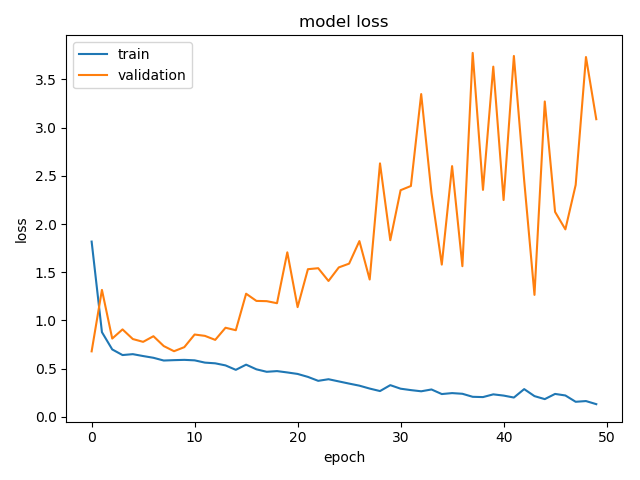
\includegraphics[width=\linewidth]{Figs/small_us_loss.jpg}
\caption{Small CNN US}
\end{subfigure}
\begin{subfigure}[b]{.45\linewidth}
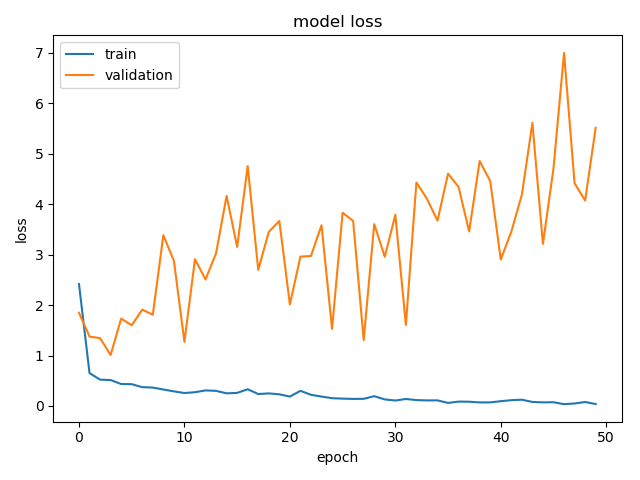
\includegraphics[width=\linewidth]{Figs/small_pat_loss.jpg}
\caption{Small CNN PAT}
\end{subfigure}

\begin{subfigure}[b]{.45\linewidth}
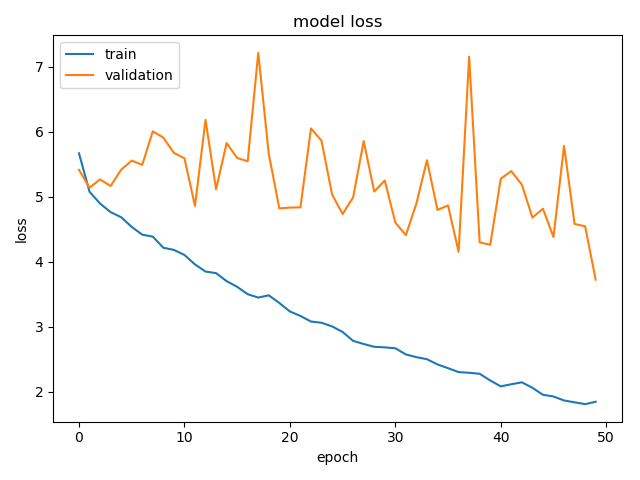
\includegraphics[width=\linewidth]{Figs/resnet_us_loss.jpg}
\caption{ResNet US}
\end{subfigure}
\begin{subfigure}[b]{.45\linewidth}
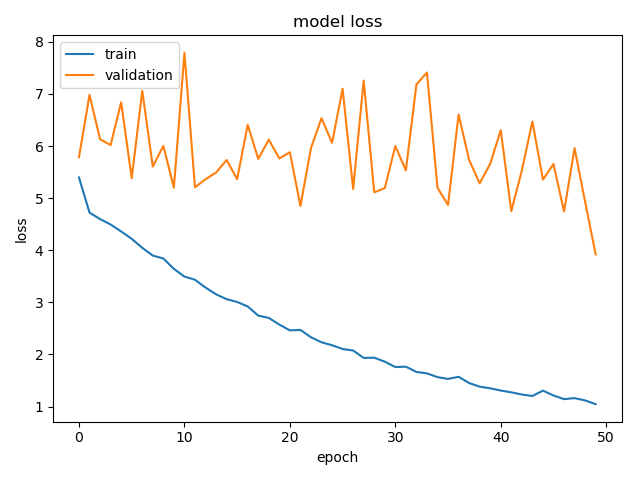
\includegraphics[width=\linewidth]{Figs/resnet_pat_loss.jpg}
\caption{ResNet PAT}
\end{subfigure}

\begin{subfigure}[b]{.45\linewidth}
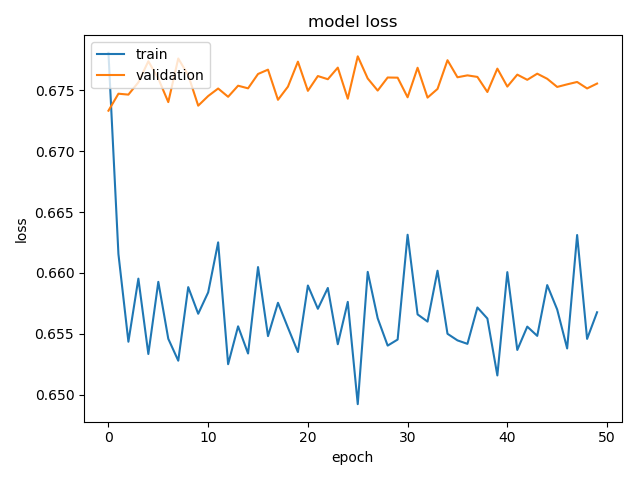
\includegraphics[width=\linewidth]{Figs/vgg_us_loss.jpg}
\caption{VGG US}
\end{subfigure}
\begin{subfigure}[b]{.45\linewidth}
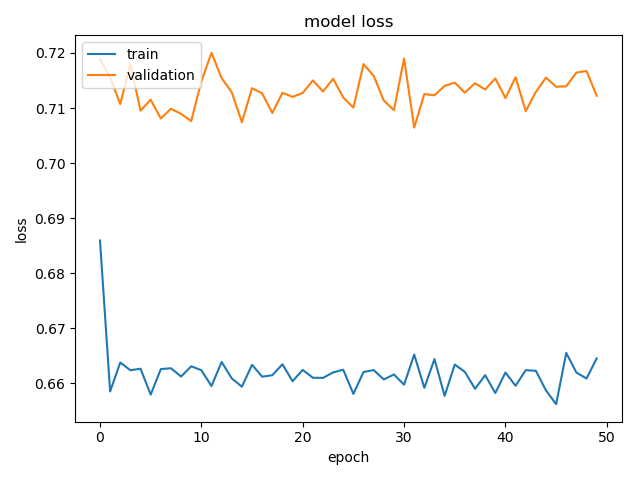
\includegraphics[width=\linewidth]{Figs/vgg_pat_loss.jpg}
\caption{VGG PAT}
\end{subfigure}

\begin{subfigure}[b]{.45\linewidth}
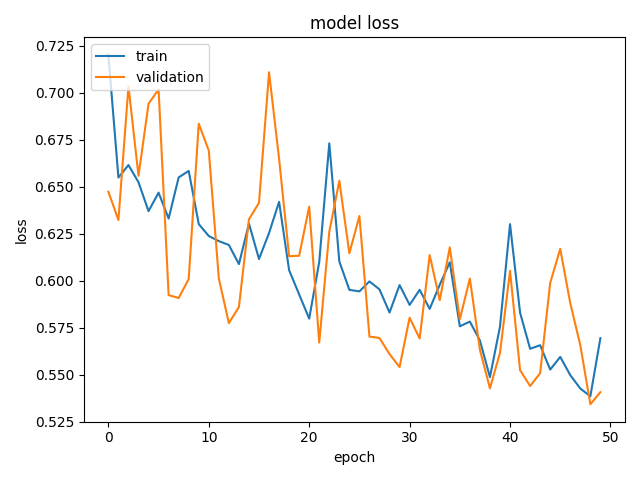
\includegraphics[width=\linewidth]{Figs/vgg_in_us_loss.jpg}
\caption{VGG-IN US}
\end{subfigure}
\begin{subfigure}[b]{.45\linewidth}
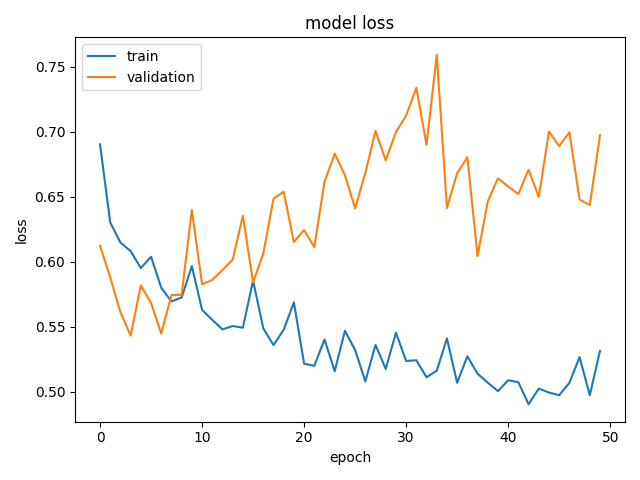
\includegraphics[width=\linewidth]{Figs/vgg_in_pat_loss.jpg}
\caption{VGG-IN PAT}
\end{subfigure}
\caption{Model loss}
\label{fig:loss}
\end{figure}

\begin{figure}
\centering
\begin{subfigure}[b]{.45\linewidth}
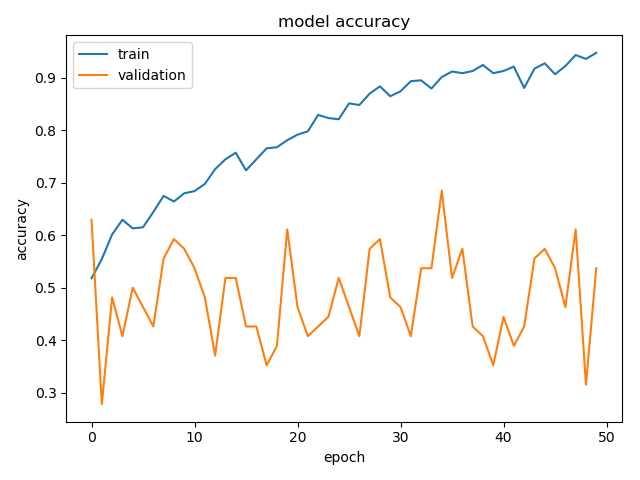
\includegraphics[width=\linewidth]{Figs/small_us_acc.jpg}
\caption{Small CNN US}
\end{subfigure}
\begin{subfigure}[b]{.45\linewidth}
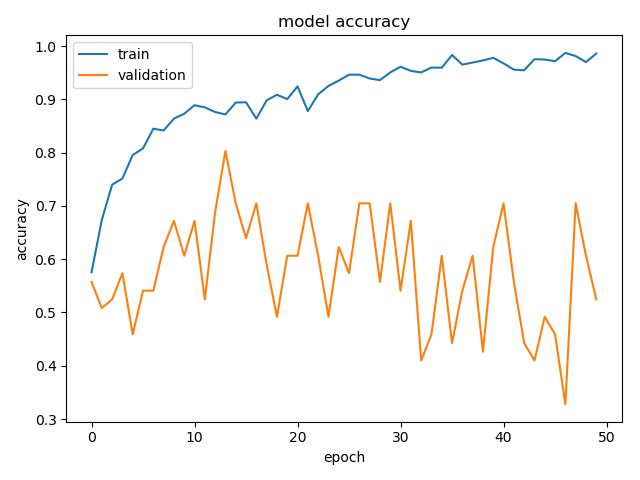
\includegraphics[width=\linewidth]{Figs/small_pat_acc.jpg}
\caption{Small CNN PAT}
\end{subfigure}

\begin{subfigure}[b]{.45\linewidth}
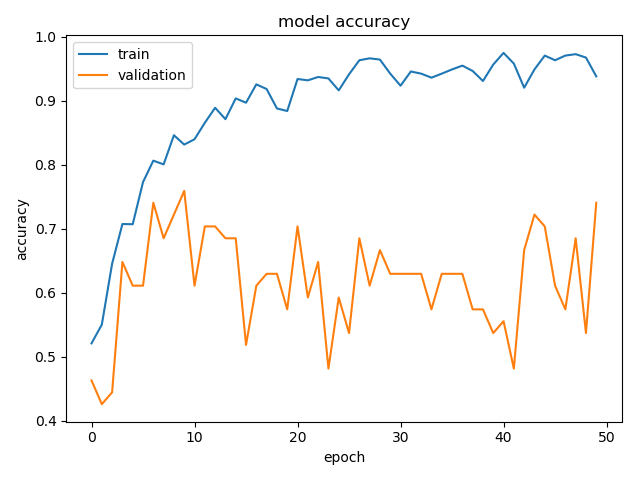
\includegraphics[width=\linewidth]{Figs/resnet_us_acc.jpg}
\caption{ResNet US}
\end{subfigure}
\begin{subfigure}[b]{.45\linewidth}
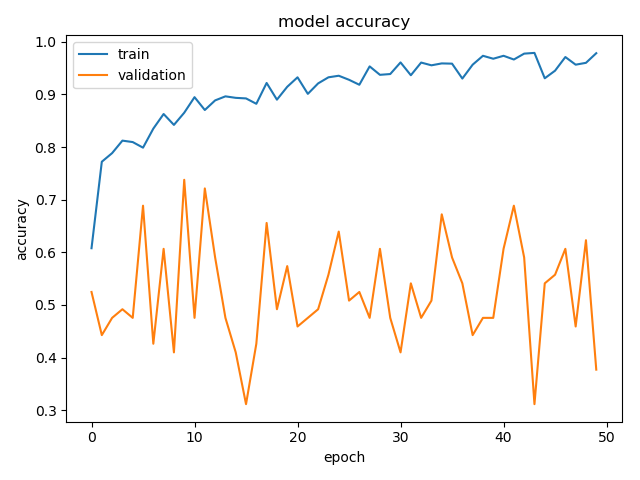
\includegraphics[width=\linewidth]{Figs/resnet_pat_acc.jpg}
\caption{ResNet PAT}
\end{subfigure}

\begin{subfigure}[b]{.45\linewidth}
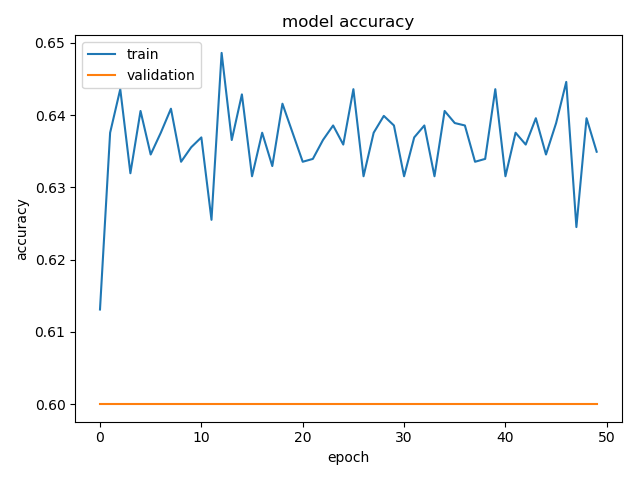
\includegraphics[width=\linewidth]{Figs/vgg_us_acc.jpg}
\caption{VGG US}
\end{subfigure}
\begin{subfigure}[b]{.45\linewidth}
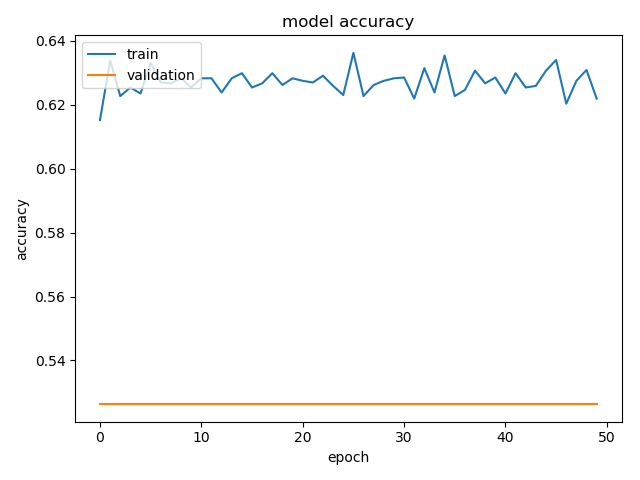
\includegraphics[width=\linewidth]{Figs/vgg_pat_acc.jpg}
\caption{VGG PAT}
\end{subfigure}

\begin{subfigure}[b]{.45\linewidth}
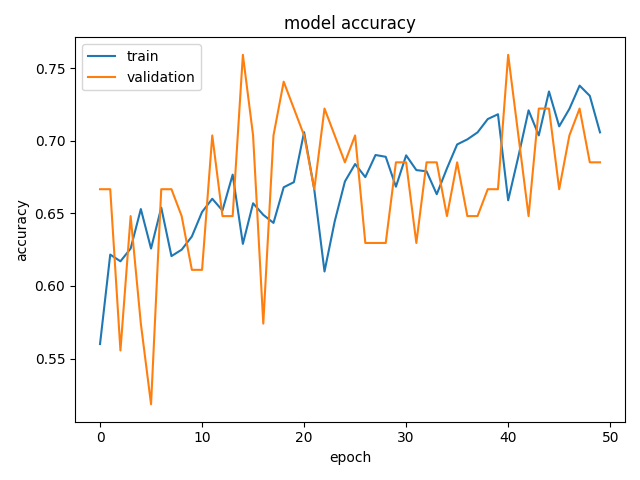
\includegraphics[width=\linewidth]{Figs/vgg_in_us_acc.jpg}
\caption{VGG-IN US}
\end{subfigure}
\begin{subfigure}[b]{.45\linewidth}
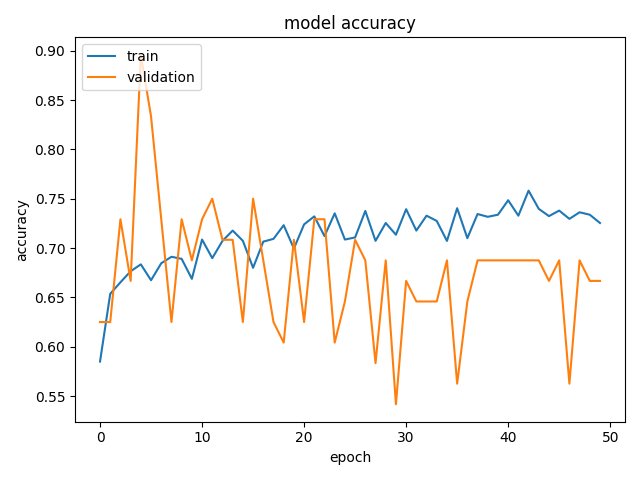
\includegraphics[width=\linewidth]{Figs/vgg_in_pat_acc.jpg}
\caption{VGG-IN PAT}
\end{subfigure}
\caption{Model accuracy}
\label{fig:acc}
\end{figure}

The learning process of a neural network can be investigated through training curves \citep{Anzanello2011}. Training and validation loss and accuracy are reported and ploted in Fig.\,\ref{fig:loss} and Fig.\,\ref{fig:acc}. 


\section{Discussion}
\label{result_discussion}

For Small CNN model, even though the training loss is decreasing over epoch, the validation loss is increasing (Fig.\,\ref{fig:loss} (A) (B)). This model is not generalizing to fit unseen validation data. For ResNet model, the decrease of training and validation loss (Fig.\,\ref{fig:loss} (C) (D)) indicates that ResNet could improve from training (although very noisy). VGG model has almost the same depth as ResNet, 19 layers versus 18 layers. Yet, the convergence of training and validation loss is very poor. We do not see a decrease in training and validation loss (Fig.\,\ref{fig:loss} (E) (F)). VGG-IN model uses a set of pre-trained weights from ImageNet \citep{imagenet_cvpr09} in convolutional layers, only the fully-connected layers and classification layer are trained. VGG-IN model shows decreases in training and validation loss on US dataset (Fig.\,\ref{fig:loss}), but on PAT dataset (Fig.\,\ref{fig:loss} (H)) only training loss decreases.

All models perform poorly in terms of accuracy on the US and PAT dataset. The validation accuracy of all models do not show a consistent improvement over epoch (Fig.\,\ref{fig:acc}). Note the large gap between training and validation curves. This indicates that the training dataset is unrepresentative, which means the training dataset does not provide sufficient information to learn the problem. We may have too few examples in the training dataset, or the training dataset may not be a good representation. From the noisy validation curves, we can conclude that the validation dataset is also unrepresentative. A unrepresentative validation set means that it does not provide sufficient information to evaluate the ability of the model to generalize. This could occur when the validation dataset has too few examples.

Medical images are naturally difficult to acquire. By machine learning standard, which often requires thousands or even millions of samples, our dataset is considered extremely small. In addition, the US and PAT scans are very noisy and have lots of artifacts. The low quality of images makes it more challenging for neural networks to pick up important features. With additional data come to hand, we hope to see an improvement on the models' performance.

\section{Experiments with other datasets}
\label{result_other}

\begin{figure}[h]
\centering
\begin{subfigure}[b]{.2\linewidth}
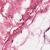
\includegraphics[width=\linewidth]{Figs/8864_idx5_x1251_y1651_class0.png}
\end{subfigure}
\begin{subfigure}[b]{.2\linewidth}
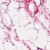
\includegraphics[width=\linewidth]{Figs/8864_idx5_x1201_y1801_class0.png}
\end{subfigure}
\begin{subfigure}[b]{.2\linewidth}
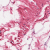
\includegraphics[width=\linewidth]{Figs/8864_idx5_x1201_y1701_class0.png}
\end{subfigure}
\begin{subfigure}[b]{.2\linewidth}
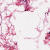
\includegraphics[width=\linewidth]{Figs/8864_idx5_x1151_y1701_class0.png}
\end{subfigure}

\begin{subfigure}[b]{.2\linewidth}
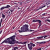
\includegraphics[width=\linewidth]{Figs/8864_idx5_x1851_y2251_class1.png}
\end{subfigure}
\begin{subfigure}[b]{.2\linewidth}
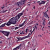
\includegraphics[width=\linewidth]{Figs/8864_idx5_x1801_y2701_class1.png}
\end{subfigure}
\begin{subfigure}[b]{.2\linewidth}
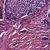
\includegraphics[width=\linewidth]{Figs/8864_idx5_x1801_y2651_class1.png}
\end{subfigure}
\begin{subfigure}[b]{.2\linewidth}
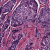
\includegraphics[width=\linewidth]{Figs/8864_idx5_x1801_y2551_class1.png}
\end{subfigure}
\caption{Examples from IDC Breast Cancer Dataset}
\label{IDC}
\end{figure}

\begin{figure}[h]
\centering
\begin{subfigure}[b]{.2\linewidth}
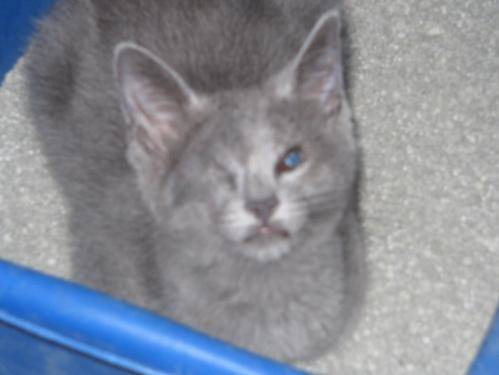
\includegraphics[width=\linewidth]{Figs/cat450.jpg}
\end{subfigure}
\begin{subfigure}[b]{.2\linewidth}
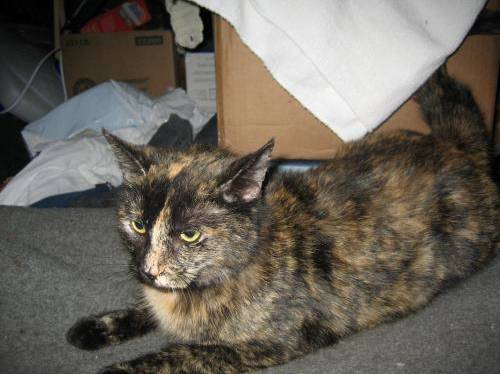
\includegraphics[width=\linewidth]{Figs/cat1921.jpg}
\end{subfigure}
\begin{subfigure}[b]{.2\linewidth}
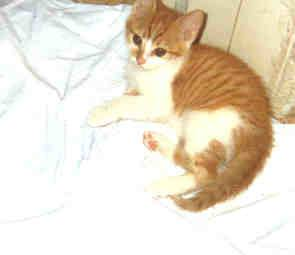
\includegraphics[width=\linewidth]{Figs/cat1412.jpg}
\end{subfigure}
\begin{subfigure}[b]{.2\linewidth}
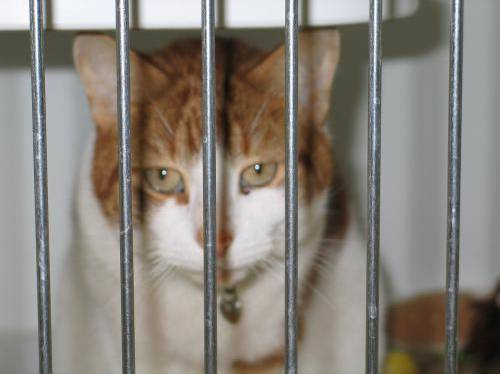
\includegraphics[width=\linewidth]{Figs/cat1168.jpg}
\end{subfigure}

\begin{subfigure}[b]{.2\linewidth}
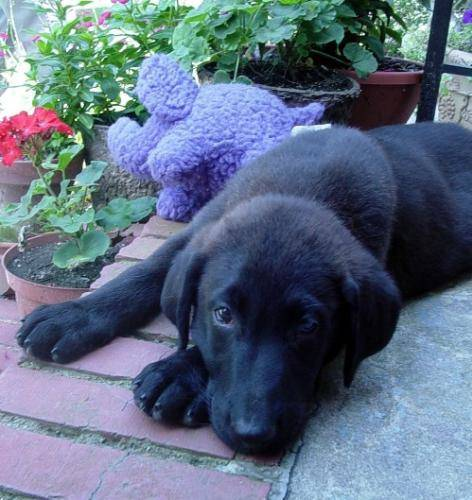
\includegraphics[width=\linewidth]{Figs/dog876.jpg}
\end{subfigure}
\begin{subfigure}[b]{.2\linewidth}
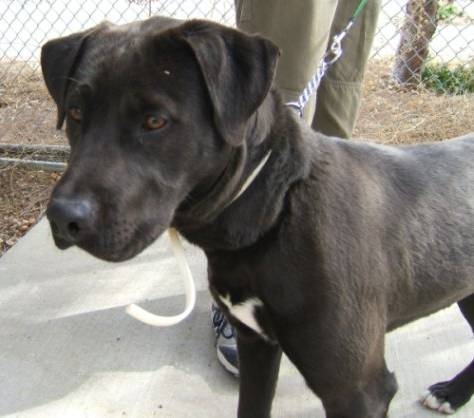
\includegraphics[width=\linewidth]{Figs/dog508.jpg}
\end{subfigure}
\begin{subfigure}[b]{.2\linewidth}
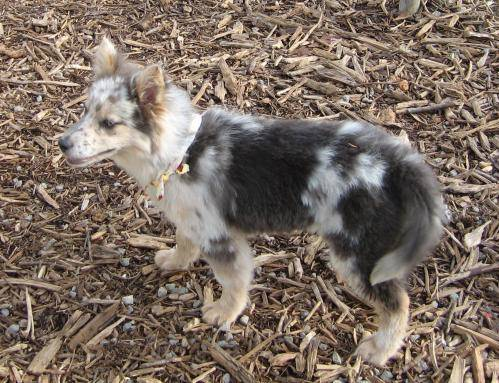
\includegraphics[width=\linewidth]{Figs/dog4133.jpg}
\end{subfigure}
\begin{subfigure}[b]{.2\linewidth}
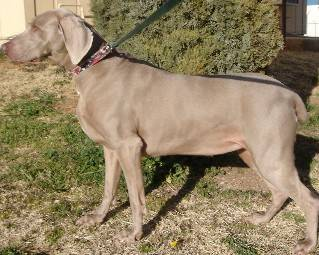
\includegraphics[width=\linewidth]{Figs/dog1178.jpg}
\end{subfigure}
\caption{Examples from Cats vs. Dogs Dataset}
\label{catdog}
\end{figure}

Due to the poor performance in experiments with our dataset, to verify the capabilities of these neural network models, they are trained on two other classification datasets, IDC Breast Cancer Dataset \citep{Janowczyk2016} (Fig.\,\ref{IDC}) and Dogs vs. Cats Dataset \citep{catdog}  (Fig.\,\ref{catdog}).


Table \ref{stats} shows the number of images in the datasets. The models are trained for 10 epoch on the IDC Breast Cancer Dataset and 30 epoch on the Dogs vs. Cats Dataset.
\begin{table}[h]
\centering
\begin{tabular}{ |p{3cm}||p{3cm}|p{3cm}|  }
 \hline
 Class       & Training set & Validation set\\
 \hline
 \hline
 IDC class 0   & 179,343   &  68,549 \\
 IDC class 1  & 71,609  & 27,763\\
 \hline
 Cat   & 10,499  &  2,003\\
 Dog  & 10,499  &  2,003\\
 \hline
\end{tabular}
\caption{Number of images in each set}
\label{stats}
\end{table}


\begin{table}[h]
\centering
\begin{tabular}{ |p{4cm}||p{3cm}|p{3cm}|p{3cm}|  }
 \hline
 Model       & Accuracy & Class 0 $F_1$ score & Class 1 $F_1$ score\\
 \hline
 \hline
 Small Breast   & \textbf{0.89}  & \textbf{0.92} &  \textbf{0.80}\\
 ResNet Breast  & 0.88  & \textbf{0.92} &  \textbf{0.80}\\
 VGG Breast      & 0.71  & 0.83 &  0\\
 VGG-IN breast & 0.85 & 0.90 & 0.73 \\
 \hline
 Small CatDog   & \textbf{0.93}  & \textbf{0.93} &  \textbf{0.93}\\
 ResNet CatDog  & \textbf{0.93}  & \textbf{0.93} &  \textbf{0.93}\\
 VGG CatDog      & 0.50  & 0.67 &  0\\
 VGG-IN CatDog  & 0.92 & 0.92 & 0.92 \\
  \hline
\end{tabular}
\caption{Model accuracy and $F_1$ score}
\label{acctable2}
\end{table}

Validation accuracy and $F_1$ score are reported in Table \ref{acctable2}. Small CNN and ResNet achieved the same accuracy and $F_1$ score on both datasets. VGG is again not able to train. Using pre-trained weights in VGG-IN is effective to improve VGG, but the performance still does not match Small CNN and ResNet. A deep neural network model such as VGG is very difficult to train due to the degradation problem. A deep network not necessarily performs better than a shallower network.

Training loss and accuracy plots are shown in Fig.\,\ref{fig:loss2}. 

\begin{figure}[h]
\centering
\begin{subfigure}[b]{.45\linewidth}
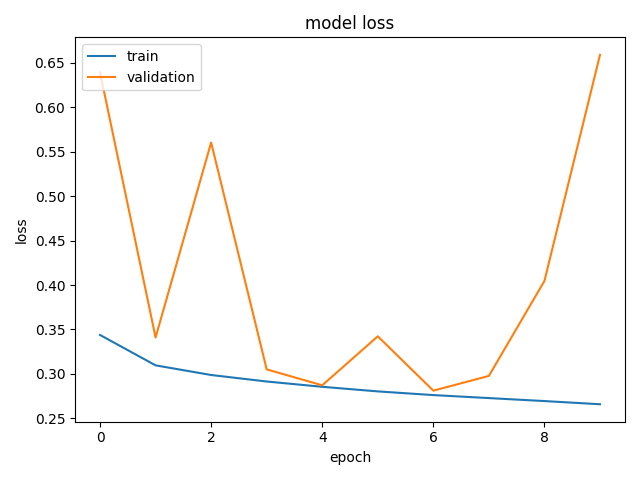
\includegraphics[width=\linewidth]{Figs/small_breast_loss.jpg}
\caption{Small Breast}
\end{subfigure}
\begin{subfigure}[b]{.45\linewidth}
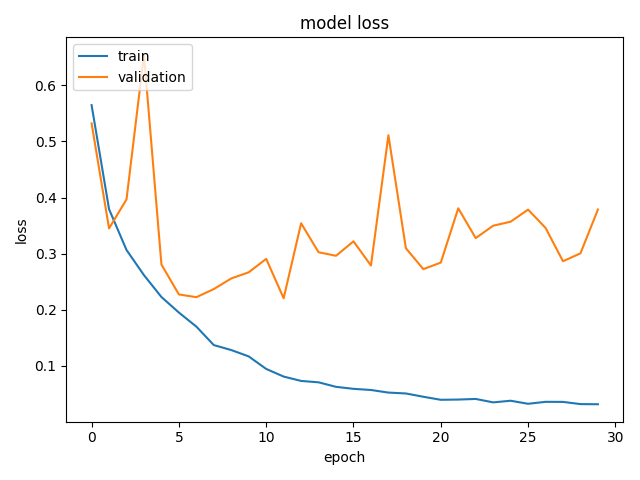
\includegraphics[width=\linewidth]{Figs/small_catdog_loss.jpg}
\caption{Small CatDog}
\end{subfigure}

\begin{subfigure}[b]{.45\linewidth}
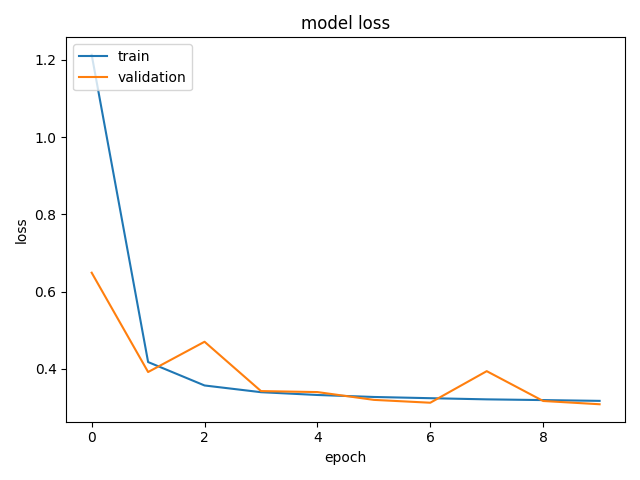
\includegraphics[width=\linewidth]{Figs/resnet_breast_loss.jpg}
\caption{ResNet Breast}
\end{subfigure}
\begin{subfigure}[b]{.45\linewidth}
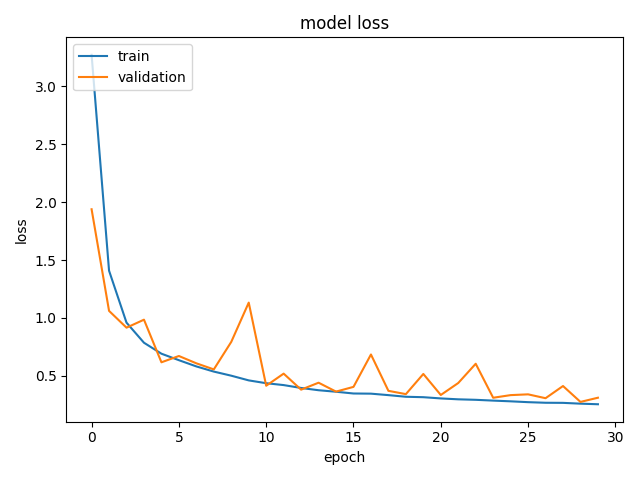
\includegraphics[width=\linewidth]{Figs/resnet_catdog_loss.jpg}
\caption{ResNet CatDog}
\end{subfigure}

\begin{subfigure}[b]{.45\linewidth}
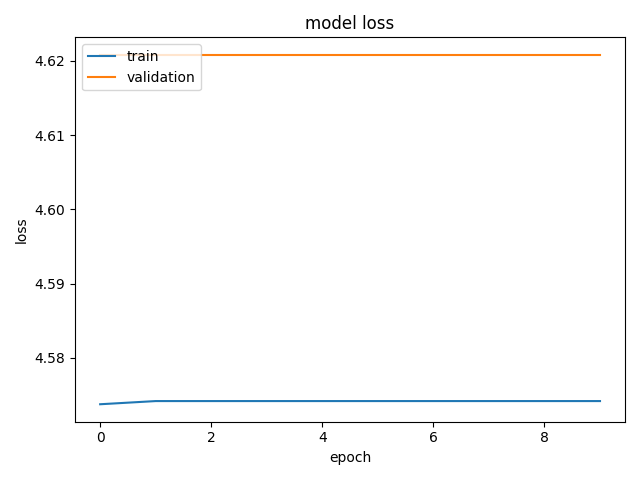
\includegraphics[width=\linewidth]{Figs/vgg_breast_loss.jpg}
\caption{VGG Breast}
\end{subfigure}
\begin{subfigure}[b]{.45\linewidth}
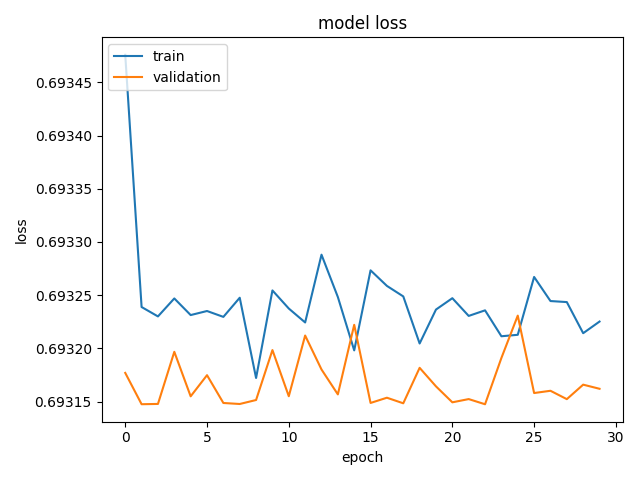
\includegraphics[width=\linewidth]{Figs/vgg_catdog_loss.jpg}
\caption{VGG CatDog}
\end{subfigure}

\begin{subfigure}[b]{.45\linewidth}
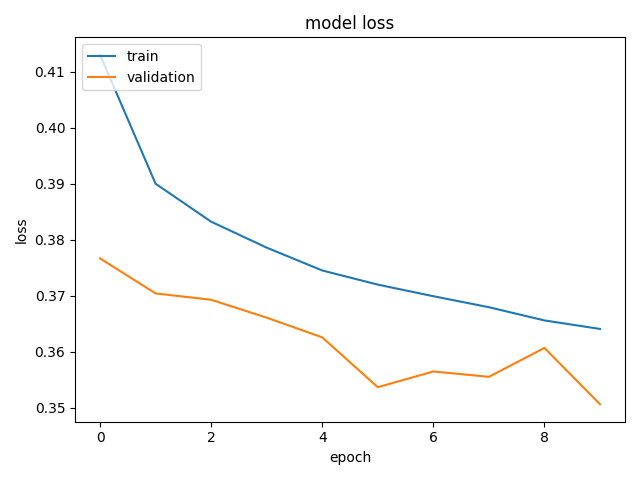
\includegraphics[width=\linewidth]{Figs/vgg_in_breast_loss.jpg}
\caption{VGG-IN Breast}
\end{subfigure}
\begin{subfigure}[b]{.45\linewidth}
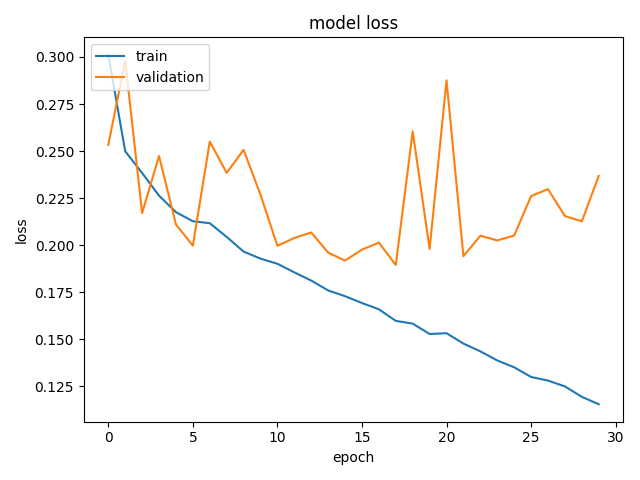
\includegraphics[width=\linewidth]{Figs/vgg_in_catdog_loss.jpg}
\caption{VGG-IN CatDog}
\end{subfigure}

\caption{Model loss}
\label{fig:loss2}
\end{figure}

\begin{figure}
\centering
\begin{subfigure}[b]{.45\linewidth}
\includegraphics[width=\linewidth]{Figs/small_breast_acc.jpg}
\caption{Small Breast}
\end{subfigure}
\begin{subfigure}[b]{.45\linewidth}
\includegraphics[width=\linewidth]{Figs/small_catdog_acc.jpg}
\caption{Small CatDog}
\end{subfigure}

\begin{subfigure}[b]{.45\linewidth}
\includegraphics[width=\linewidth]{Figs/resnet_breast_acc.jpg}
\caption{ResNet Breast}
\end{subfigure}
\begin{subfigure}[b]{.45\linewidth}
\includegraphics[width=\linewidth]{Figs/resnet_catdog_acc.jpg}
\caption{ResNet CatDog}
\end{subfigure}

\begin{subfigure}[b]{.45\linewidth}
\includegraphics[width=\linewidth]{Figs/vgg_breast_acc.jpg}
\caption{VGG Breast}
\end{subfigure}
\begin{subfigure}[b]{.45\linewidth}
\includegraphics[width=\linewidth]{Figs/vgg_catdog_acc.jpg}
\caption{VGG CatDog}
\end{subfigure}

\begin{subfigure}[b]{.45\linewidth}
\includegraphics[width=\linewidth]{Figs/vgg_in_breast_acc.jpg}
\caption{VGG-IN Breast}
\end{subfigure}
\begin{subfigure}[b]{.45\linewidth}
\includegraphics[width=\linewidth]{Figs/vgg_in_catdog_acc.jpg}
\caption{VGG-IN CatDog}
\end{subfigure}

\caption{Model accuracy}
\label{fig:acc2}
\end{figure}
